% FUNDAMENTAÇÃO TEÓRICA--------------------------------------------------------

\chapter{FUNDAMENTAÇÃO TEÓRICA}
\label{chap:fundamentacao-teorica}

Este capítulo descreve as tecnologias e conceitos centrais utilizados durante a concepção do projeto. As definições apresentadas são embasadas no material bibliográfico revisado, que serviu de apoio no desenvolvimento de um trabalho fundamentado nas teorias existentes.

\section{\textit{Raspberry Pi}}
\label{sec:raspi}

O \textit{Raspberry Pi} é uma família de computadores com arquitetura de processador ARM (\textit{Advanced RISC Machine}), desenvolvido em um único chip de silício, chamados de SoC (\textit{System on Chip}), com o tamanho de um cartão de crédito. Inicialmente, seu objetivo era promover o ensino de computação (programação) básica em escolas, principalmente públicas, de todo o mundo. Entretanto, por possuir um poder computacional razoável, uma boa quantidade de memória RAM (\textit{Random Access memory}) (a partir do modelo B, ilustrado na \autoref{fig:raspi_modelb}) e um preço relativamente baixo, passou a ser usado para outros objetivos como: console de \textit{videogame} clássico (emulação de jogos), gerencia de mídia (vídeos, fotos e músicas), estudos em eletrônica, domótica (automação residencial), internet das coisas e robótica. \citeonline{jucapereira2018aplicacoes} \par
Uma versão do sistema operacional \textit{Debian Linux}, chamada \textit{Raspbian}, foi portada para o \textit{Raspberry Pi}, levando também uma série de aplicativos e ferramentas de desenvolvimento já existentes para computadores com arquitetura x86. Desse modo, o desenvolvimento de programas se torna uma tarefa extremamente simples, já que o sistema operacional fornece a HAL (\textit{Hardware Abstraction Layer}), não sendo necessário o conhecimento específico do \textit{hardware} do \textit{Raspberry Pi}. \par
Existem várias linguagens de programação portadas para o \textit{Raspberry Pi}. As mais utilizadas para desenvolvimento de software, com bibliotecas disponíveis para interação com o \textit{hardware}, são o C/C++ e Python, porém é possível desenvolver em outras linguagens de programação, como o PHP e Java. \citeonline{jucapereira2018aplicacoes} \par

\begin{figure}[H]
	\centering
	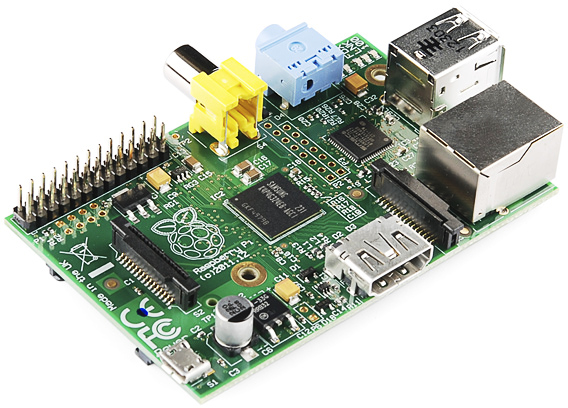
\includegraphics[width=0.6\textwidth]{figuras/raspberrypi_model_b.jpg}
	\caption{Raspberry Pi (Modelo B).}
	\fonte{ \citeonline{sparkfun2019}}
	\label{fig:raspi_modelb}
\end{figure}

\section{Servo Motor}
\label{sec:servomotor}

Um servo motor, visto na \autoref{fig:servo_g9}, é um atuador rotatório ou atuador linear, que permite um controle preciso da posição linear ou angular, velocidade e aceleração de uma carga ligada ao seu eixo. Consiste basicamente em um motor, normalmente de corrente contínua, acoplado a um sensor (potenciômetro) para ler sua posição durante o movimento, conforme ilustrado na \autoref{fig:insideaservo}. Normalmente, os motores servos são controlados por um sinal PWM (\textit{Pulse Width Modulation}). \citeonline{petruzella2009electric} \par

\begin{figure}[h]
	\centering
	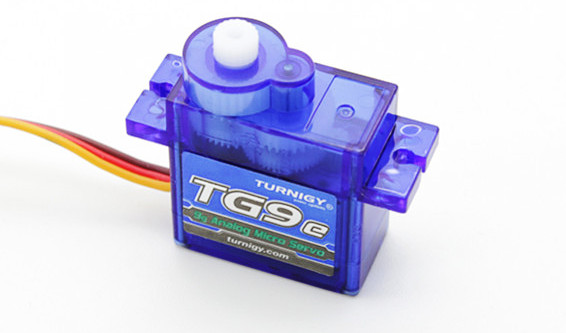
\includegraphics[width=0.6\textwidth]{figuras/servo_g9.jpg}
	\caption{Servo Micro TG9.}
	\fonte{ \citeonline{hobbyking2019}}
	\label{fig:servo_g9}
\end{figure}

O servo motor opera em malha fechada, isto é, seu controlador compara a velocidade e sua posição para gerar o próximo comando de movimento, minimizando o erro. \citeonline{petruzella2009electric}. O esquema de funcionamento do servo motor é mostrado na figura \autoref{fig:servo_closed_loop}. 

\begin{figure}[h]
	\centering
	\begin{subfigure}{.5\textwidth}
		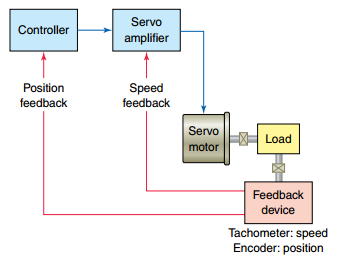
\includegraphics[width=0.95\textwidth]{figuras/servo_closed_loop.png}
		\caption{Sistema em malha fechada.}
		\fonte{ \citeonline{petruzella2009electric}}
		\label{fig:servo_closed_loop}
	\end{subfigure}%
	\begin{subfigure}{.5\textwidth}
		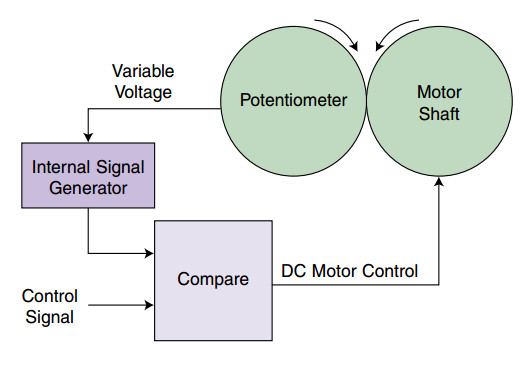
\includegraphics[width=0.95\textwidth]{figuras/inside_a_servo.jpg}
		\caption{Componentes internos.}
		\fonte{\citeonline{pinckney2006pulse}.}
		\label{fig:insideaservo}
	\end{subfigure}
	\caption{Sistema de controle de um servo motor.}
\end{figure}

\section{Modulação por Largura de Pulso - PWM}
\label{sec:pwm}

A modulação por largura de pulso é uma técnica empregada em diversas áreas da eletrônica. Sendo utilizada para controlar fontes chaveadas, velocidade de motores, luminosidade, servo motores e diversas outras aplicações. Consiste em variar o tempo em que um pulso de tensão oscila entre os níveis alto e baixo, numa taxa rápida o suficiente para que a média dos pulsos crie um valor médio de tensão efetivo, ilustrado na \autoref{fig:pwm}. É dado o nome \textbf{ciclo de trabalho} ou \textit{dutty cycle} ao valor definido pela divisão entre a largura de pulso, com a tensão em nível alto, e o período do sinal. Variar o \textit{dutty cycle} significa variar a tensão média gerada pelo sinal. Como a potência de um dispositivo é proporcional a tensão, reduzir a potência de um dispositivo operado por PWM (a exemplo, um LED ou motor DC), é o mesmo que reduzir o \textit{dutty cycle} do sinal. \citeonline{pinckney2006pulse}.

\begin{figure}[h]
	\centering
	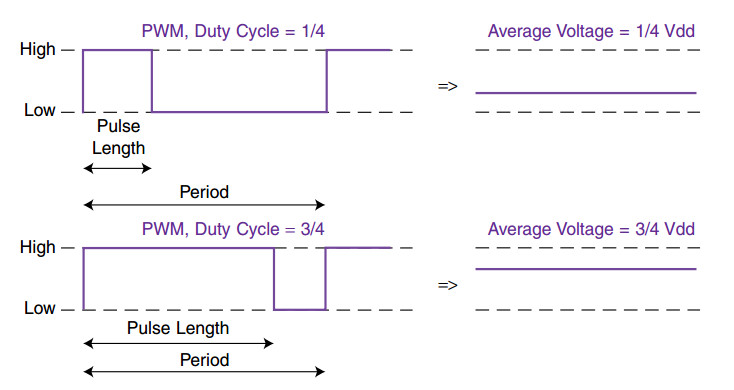
\includegraphics[width=1\textwidth]{figuras/pwm.jpg}
	\caption{Modulação por largura de pulso e tensão média resultante}
	\fonte{ \citeonline{pinckney2006pulse}}
	\label{fig:pwm}
\end{figure}

A largura de pulso pode ser calculada usando a \autoref{eq:duttycicle}.

\begin{equation}
{C} = 100 \times \frac{LP}{P}  
\label{eq:duttycicle}
\end{equation}

Onde: \textbf{C} é um valor dado em percentual, \textbf{LP} e \textbf{P} são valores dados em segundos.\par

Uma vez calculado o ciclo de trabalho, é possível calcular o valor da tensão média gerada pelo sinal através da \autoref{eq:avervoltage}.

\begin{equation}
{TM} = {TP} \times {C}
\label{eq:avervoltage}
\end{equation}

Onde: \textbf{TM} é a tensão média resultante, dado em volts, \textbf{TP} é a tensão usada na geração do pulso PWM, também dado em volts, e \textbf{\textit{C}} é o valor encontrado com a \autoref{eq:duttycicle}, dado em percentual.

\section{\textit{Smartphone} Android}
\label{sec:android}

O \textit{smartphone} é um dispositivo móvel que mescla recursos de um telefone celular (receber e efetuar chamadas, mensagens de texto curto, dentre outros) e recursos de um computador pessoal, garantindo a possibilidade de se instalar novos aplicativos, agregando diferentes funcionalidades ao aparelho.\par

O \textit{Android} é um sistema operacional de código livre, baseado em núcleo \textit{Linux} (responsável por gerenciar dispositivos de entrada e saída, memória, processos e segurança), marcado em vermelho na \autoref{fig:androidsysarch}. É desenvolvido por uma das maiores empresas de tecnologia da atualidade, a Google \citeonline{ronamadeo2018}. Sua interface com o usuário é baseada na manipulação direta, isto é, apresenta continuamente o objeto de interesse, permitindo sua manipulação, usando recursos que correspondem proximamente ao mundo físico \citeonline{barbosa2010interaccao}. Atualmente, o sistema operacional \textit{Android} pode ser encontrado em outros aparelhos como relógios, televisores e dispositivos gerenciadores de mídia \citeonline{androidcom2019}. \par

\begin{figure}[H]
	\centering
%	\begin{subfigure}{.5\textwidth}
		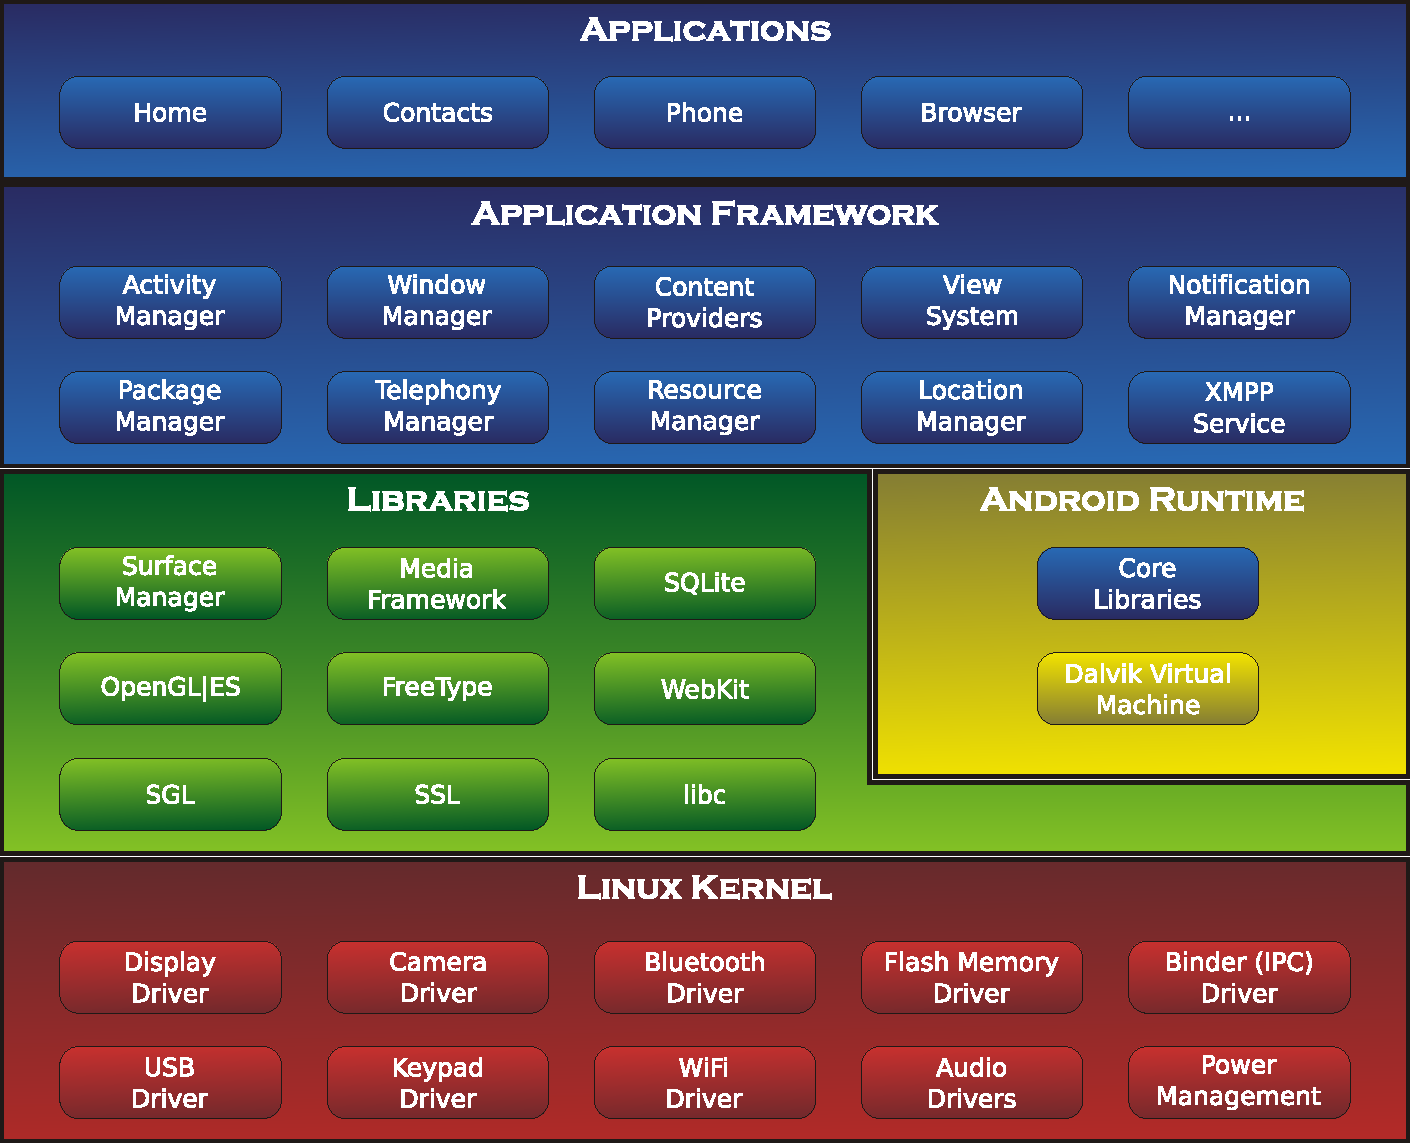
\includegraphics[width=0.7\textwidth]{figuras/android_sys_arch.pdf}
		\caption{Arquitetura do sistema operacional Android.}
		\fonte{ \citeonline{brady2008anatomy}.}
		\label{fig:androidsysarch}
%	\end{subfigure}%
%	\begin{subfigure}{.5\textwidth}
%		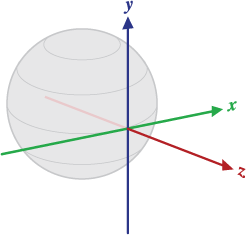
\includegraphics[width=0.95\textwidth]{figuras/axis_globe.png}
%		\caption{em relação ao globo terrestre.}
%		\label{fig:axisglobe}
%	\end{subfigure}
%	\caption{Sistema operacional Android.}
\end{figure}

Boa parte dos \textit{smartphones}, vendidos atualmente com o sistema operacional \textit{Android}, possuem uma gama de sensores embutidos, capazes de fornecer dados, com um grau de precisão aceitável, relativos a orientação e movimento do aparelho e até condições do ambiente, como exemplo: iluminação, pressão atmosférica e umidade do ar \citeonline{androidcom2019}. Esses sensores encontram-se divididos em três grupos básicos na API de desenvolvimento fornecida pelo \textit{Android}: Sensores \textbf{Ambientais}, que podem ser utilizados em aplicações simples, como coletar o nível de iluminação do ambiente, a umidade e temperatura, para calcular o ponto de orvalho (condição em que a água em vapor presente num ambiente se condensa, tornando-se o orvalho); Sensores de \textbf{Posição} e de \textbf{Movimento}, que podem ser usados em aplicações, a exemplo de jogos que utilizam a aceleração da gravidade para inferir movimentos complexos do usuário como rotações, sacudidas e inclinações do aparelho. Sendo este último grupo, o ponto de interesse para o trabalho, detalhado adiante.\par

\subsection{Sensores de Movimento}
\label{subsec:motionsensors}

A API do \textit{Android} oferece vários sensores que permitem sentir o movimento de um dispositivo. Dentre eles, os mais utilizados são os sensores de gravidade, aceleração linear e vetor de rotação. Eles podem ser implementados em \textit{hardware} ou \textit{software} (baseando-se em dados fornecidos por outros sensores, implementados em \textit{hardware}). Bem como os sensores \textbf{acelerômetro} e \textbf{giroscópio}, que sempre são implementados em \textit{hardware}. Todos eles, descrevem o movimento do dispositivo, através de uma estrutura de dados em formato matricial (\textit{array} com mais de uma dimensão).\par

De forma geral, os sensores usam um sistema de coordenadas com três eixos para expressar os dados. Para a maioria dos sensores da API, o sistema de coordenadas é definido relativo a tela do dispositivo, quando segurado na orientação padrão (porta retrato para celulares e paisagem para \textit{tablets}), como mostrado na \autoref{fig:axisdevice}. Dessa forma, o eixo $X$ é horizontal e aponta para a direita, o eixo $Y$ é vertical apontando para cima e o eixo $Z$, perpendicular a tela do dispositivo, estando seus valores positivos sobre a tela, e os negativos sob a tela. Um ponto importante a ser notado, é que a orientação do sistema de eixos não muda, quando o dispositivo é segurado de maneira diferente da sua orientação padrão.\par

\begin{figure}[H]
	\centering
	\begin{subfigure}{.5\textwidth}
		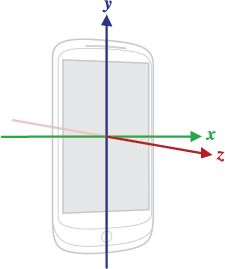
\includegraphics[width=0.85\textwidth]{figuras/axis_device.png}
		\caption{em relação ao aparelho.}
		\label{fig:axisdevice}
	\end{subfigure}%
	\begin{subfigure}{.5\textwidth}
		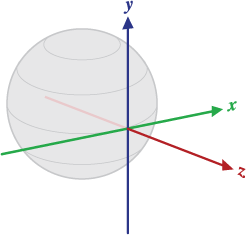
\includegraphics[width=0.95\textwidth]{figuras/axis_globe.png}
		\caption{em relação ao globo terrestre.}
		\label{fig:axisglobe}
	\end{subfigure}
	\caption{Sistema de coordenadas.}
	\fonte{ \citeonline{google2019devsensors}.}
\end{figure}

O sensor \textbf{vetor de rotação} representa a orientação do aparelho como uma combinação de um ângulo e um eixo, no qual o dispositivo rotacionou com um ângulo $\theta$ em torno de um eixo ($x$, $y$ ou $z$) \citeonline{google2019devsensors}. \par
Os três componentes do vetor de rotação são expressos como:\\

\begin{equation}
\Delta_x = x \times sen(\frac{\theta}{2})
\label{eq:vec_rot_x}
\end{equation}

\begin{equation}
\Delta_y = y \times sen(\frac{\theta}{2})
\label{eq:vec_rot_y}
\end{equation}

\begin{equation}
\Delta_z = z \times sen(\frac{\theta}{2})
\label{eq:vec_rot_z}
\end{equation}

Onde, a magnitude do vetor de rotação é expressa por $sen(\frac{\theta}{2})$, e sua direção é a mesma do eixo de rotação ao qual está multiplicando.\par

O sistema de coordenada de referência é definido como uma base ortogonal direta, isto é, os seus vetores são mutuamente ortogonais, como mostrado na \autoref{fig:axisglobe}, e possui as seguintes características:\par
\begin{itemize}
\item O eixo $X$ é definido como o produto vetorial dos eixos $Y$ e $Z$, é tangente à superfície terrestre, no local onde o dispositivo se encontra, e aponta aproximadamente para o leste.\par

\item O eixo $Y$ é tangente à superfície terrestre, no local onde o dispositivo se encontra, e aponta para o norte magnético. \par

\item O eixo $Z$ aponta para o céu e é perpendicular ao solo.
\end{itemize}